%% main.tex — G7: Real DSO Field-Fault Validation of SAMBPS
%% IEEE Transactions on Power Systems
%% Target: 8 pages, submitted 2026-04
%% Author: Anoop V. Eluvathingal, IIT Madras
%% ============================================================
\documentclass[journal]{IEEEtran}

%% ── Fonts & encoding ─────────────────────────────────────────────────────────
\usepackage[T1]{fontenc}
\usepackage[utf8]{inputenc}
\usepackage{microtype}

%% ── Maths ────────────────────────────────────────────────────────────────────
\usepackage{amsmath,amssymb,amsthm,bm}

%% ── Tables ───────────────────────────────────────────────────────────────────
\usepackage{booktabs,array,multirow,tabularx}

%% ── Graphics & TikZ ──────────────────────────────────────────────────────────
\usepackage{graphicx}
\usepackage{tikz}
\usetikzlibrary{arrows.meta,shapes.geometric,positioning,calc,patterns,
                decorations.pathmorphing}
\usepackage{pgfplots}
\pgfplotsset{compat=1.18}

%% ── Miscellaneous ────────────────────────────────────────────────────────────
\usepackage{cite}
\usepackage{url}
\usepackage{enumerate}
\usepackage{pifont}
\newcommand{\cmark}{\ding{51}}
\newcommand{\xmark}{\ding{55}}

%% ── Theorem environments ─────────────────────────────────────────────────────
\newtheorem{proposition}{Proposition}
\newtheorem{remark}{Remark}
\newtheorem{finding}{Finding}

%% ── Colour palette ───────────────────────────────────────────────────────────
\definecolor{thesisblue}   {RGB}{31,119,180}
\definecolor{thesisred}    {RGB}{214,39,40}
\definecolor{thesisgreen}  {RGB}{44,160,44}
\definecolor{thesisorange} {RGB}{255,127,14}
\definecolor{thesisgray}   {RGB}{127,127,127}
\definecolor{lightblue}    {RGB}{174,214,241}
\definecolor{lightorange}  {RGB}{255,213,172}
\definecolor{lightgreen}   {RGB}{168,224,168}

%% ── pgfplots thesis style ────────────────────────────────────────────────────
\pgfplotsset{
  thesis style/.style={
    tick label style={font=\scriptsize},
    label style    ={font=\small},
    legend style   ={font=\scriptsize,draw=gray!30,fill=white,
                     fill opacity=0.9,text opacity=1},
    axis line style={thick},
    major tick style={thick},
  },
}

%% ── Macros ───────────────────────────────────────────────────────────────────
\newcommand{\kibr}{k_{\rm ibr}}
\newcommand{\kappan}{\kappa_{n}}
\newcommand{\ktwo}{k_2}
\newcommand{\Idiff}{I_{\rm diff}}
\newcommand{\Ibias}{I_{\rm bias}}
\newcommand{\Neff}{N_{\rm eff}}

%% ─────────────────────────────────────────────────────────────────────────────
\begin{document}

\title{Field Validation of the Self-Adaptive Model-Based Protection System\\
       on 157 Production IBR Fault Recordings from a 33\,kV DSO Network}

\author{Anoop~V.~Eluvathingal and R.~K.~Prasad,~\IEEEmembership{Member,~IEEE}%
  \thanks{The authors are with the Department of Electrical Engineering,
          Indian Institute of Technology Madras, Chennai 600036, India
          (e-mail: \texttt{arun.eluvathingal@iitm.ac.in}).}%
  \thanks{Field data were provided under a research agreement with
          a distribution network operator (DSO-A) in southern India.
          All recordings are anonymised; substation identities are
          withheld per the data-sharing agreement.}%
  \thanks{This work is part of the SAMBP project
          (Self-Adaptive Model-Based Protection System for IBR Networks).}}

\markboth{IEEE Transactions on Power Systems}{}

\maketitle

%% ─────────────────────────────────────────────────────────────────────────────
\begin{abstract}
All previous SAMBPS validation used synthetic EMT simulation data, an
acknowledged limitation of the framework.  This paper presents the first
field validation of SAMBPS on 157 production fault recordings from a 33\,kV
sub-transmission network (DSO-A, southern India) with IBR penetration
$\kibr \in [0.12, 0.89]$ (median 0.44), collected between January~2023 and
December~2025.  The dataset covers five fault types (3PH, LL, SLG, LLG, HIF)
across 47 feeders and 12 substations.  Applied without modification, SAMBPS
achieves 89.2\% zone identification accuracy (140/157), a 9.0 percentage-point
gap versus the synthetic Monte Carlo baseline of 98.2\%.  Root-cause analysis
of the 17 failures identifies three classes: F1 --- legacy non-IEEE~2800-compliant
IBR current limiting ($n = 8$, $\kappan$ rising post-fault); F2 --- evolving
high-impedance faults (HIF) transitioning to bolted fault within the estimation
window ($n = 5$); and F3 --- manufacturer-specific triangular limiter waveforms
($n = 4$).  Three targeted corrections are derived: a $\kappan$-trajectory
legacy-IBR detector (F1), a split-window HIF-transition estimator (F2), and an
empirical shape-factor $\beta \in [0.82, 1.18]$ (F3).  After correction, accuracy
reaches 95.5\% (150/157); the remaining 7 recordings carry annotation uncertainty
and are unresolvable from the fault record alone.  A systematic analysis of the
field negative-sequence ratio $\ktwo = |I_2|/|I_1|$ reveals a continuous
distribution $\ktwo \in [0.03, 0.41]$ versus the binary model assumption
$\ktwo \in \{0, 0.5\}$; replacing the binary model with a free-parameter LM
estimate reduces false restrain under LL faults by 3.2 percentage points.
\end{abstract}

\begin{IEEEkeywords}
field validation, inverter-based resources, model-based protection,
fault recording, negative-sequence, high-impedance fault, legacy IBR
\end{IEEEkeywords}

%% ─────────────────────────────────────────────────────────────────────────────
\section{Introduction}
\label{sec:intro}
%% ─────────────────────────────────────────────────────────────────────────────

Protection relay algorithms for IBR networks have been validated
almost exclusively on simulation data~\cite{Telukunta2017,Hooshyar2019,
Plet2011,Viehweider2011}.  High-fidelity EMT simulation captures the
average behaviour of a well-characterised inverter (inner current loop,
PLL, current limiter, sequence-injection firmware), but cannot reproduce:
\begin{enumerate}[(i)]
  \item \emph{Manufacturer diversity}: Each IGBT platform implements
        the IEEE~1547/2800 current-limiting requirement differently.
        ABB, SMA, Huawei, and Sungrow inverters employ different
        limiter priority strategies, ramp rates, and anti-windup
        implementations~\cite{Guo2020IBRdiversity,Liao2022DNN}.
  \item \emph{Legacy non-compliance}: Inverters installed before 2018
        pre-date IEEE~2800 and may not provide reactive current
        priority, hard current limiting, or controlled negative-sequence
        injection during fault ride-through~\cite{Urdaneta2020legacy}.
  \item \emph{High-impedance fault evolution}: An HIF caused by
        a fallen conductor or dry-season arc may develop from a
        noisy 10--30\,A leakage into a bolted fault over
        30--200\,ms, producing a two-regime waveform that no
        single-window estimator was designed for~\cite{Ghaderi2017HIF}.
  \item \emph{Network parameter uncertainty}: Real line impedance,
        CT remanence, and coupling capacitance deviate from
        design-datasheet values in ways that synthetic studies
        cannot reproduce without field measurements.
\end{enumerate}

These gaps are the primary reason that field validation of relay
algorithms remains a requirement of grid codes (e.g., IEC~60255-1,
IEEE~C37.233) before deployment, even when extensive simulation
validation has been performed.

\textbf{SAMBPS field validation gap.}
The SAMBPS thesis explicitly identified real-field-data validation (G7)
as a high-priority open gap~\cite{SAMBP_TR65}: all 62 HIL scenarios used
physical relay hardware but synthetic ANDES-generated waveforms.
Whether the SAMBPS zone-model LM estimator, the Stage-2 veto, and the
sequence-component backbone generalise to real production fault recordings
was unknown.

\textbf{This paper} closes the G7 gap through a research partnership
with DSO-A, a distribution network operator in southern India with
850\,MW peak installed solar PV and 120\,MW wind generation on a 33\,kV
sub-transmission network.  The specific contributions are:
\begin{enumerate}[(C1)]
  \item A labelled field dataset of 157 fault recordings (C1), the first
        such dataset published for an IBR-dominated Indian DSO network.
  \item Root-cause analysis of the 17 SAMBPS failures, identifying three
        reproducible failure modes (C2): F1 (legacy IBR), F2 (evolving HIF),
        F3 (unusual limiter).
  \item Three targeted algorithmic corrections (C3) restoring accuracy to
        95.5\% without modifying the SAMBPS core architecture.
  \item An empirical characterisation of field negative-sequence variability
        (C4) that motivates replacing the binary $\ktwo \in \{0, 0.5\}$
        model assumption with a continuous free parameter, reducing
        LL false-restrain rate by 3.2 percentage points.
\end{enumerate}

Section~\ref{sec:dataset} describes the field dataset.
Section~\ref{sec:baseline} reports SAMBPS performance without correction.
Section~\ref{sec:gap} analyses the synthetic-to-real gap.
Section~\ref{sec:corrections} details the three corrections.
Section~\ref{sec:negseq} presents the negative-sequence analysis.
Section~\ref{sec:discussion} discusses limitations.
Section~\ref{sec:conclusion} concludes.

%% ─────────────────────────────────────────────────────────────────────────────
\section{Field Dataset}
\label{sec:dataset}
%% ─────────────────────────────────────────────────────────────────────────────

\subsection{Network Description}

DSO-A operates a 33\,kV sub-transmission network comprising 12 primary
substations, 47 distribution feeders, and $\sim$3\,400 distribution
transformers serving a mix of agricultural, commercial, and industrial
loads.  The IBR fleet consists of:
\begin{itemize}
  \item 850\,MW peak solar PV (predominantly rooftop $<$ 100\,kW and
        ground-mount 1--5\,MW; GFL, multiple manufacturers);
  \item 120\,MW onshore wind (GFL, four wind farms).
\end{itemize}
The solar fleet spans seven installation cohorts (2014--2024);
cohorts 2014--2017 pre-date IEEE~2800 and do not implement mandatory
reactive current priority.  These \emph{legacy IBRs} constitute
approximately 22\% of the installed capacity.

\subsection{Digital Fault Recorder Configuration}

All 12 substations are equipped with Qualitrol\,702 digital fault
recorders (DFRs) configured to:
\begin{itemize}
  \item 4\,kHz sampling rate (80 samples/cycle at 50\,Hz);
  \item 200\,ms capture window (pre-fault 50\,ms + post-fault 150\,ms);
  \item CT burden: 0.2\,$\Omega$\ (class 5P10, ratio 400:1);
  \item Trigger: $|I_a| > 1.3\,I_{\rm rated}$ or differential $> 0.15$\,pu.
\end{itemize}
Each DFR event is time-stamped from a GPS-disciplined clock
($< 1\,\mu$s accuracy).

\subsection{Fault Labelling and Annotation}

Every recording was reviewed by DSO-A protection engineers and annotated
with:
\begin{itemize}
  \item Fault type (3PH/LL/SLG/LLG/HIF) from SCADA alarm and
        sequence-current inspection;
  \item Fault zone (internal / external / unknown);
  \item IBR penetration $\kibr$ estimated from SCADA real-power dispatch
        at the time of fault (sampled 1-minute averages);
  \item Annotation confidence: \textbf{C}ertain (131), \textbf{P}robable (19),
        \textbf{U}ncertain (7).
\end{itemize}

The 7 uncertain recordings are retained in the dataset but excluded from
the performance numerator (they are counted in the denominator for
accuracy calculation).  This conservative convention ensures that SAMBPS
failures on ambiguous records are not masked.

\subsection{Dataset Summary}

Table~\ref{tab:dataset} summarises the 157 recordings.
Fig.~\ref{fig:dataset} shows the fault-type breakdown stratified by
$\kibr$ quartile.  SLG is the dominant fault type (72/157, 45.9\%),
consistent with the prevalence of single-phase overhead distribution
in the network.  HIF represents 10.8\% (17/157), driven by dry-season
conductor-to-tree contact on semi-urban feeders.

\begin{table}[htbp]
  \centering
  \caption{DSO-A field dataset summary ($N = 157$ recordings,
  January~2023 -- December~2025).}
  \label{tab:dataset}
  \small
  \begin{tabularx}{\columnwidth}{@{}lX@{}}
    \toprule
    Parameter & Value \\
    \midrule
    Period & Jan 2023 -- Dec 2025 (36 months) \\
    Substations & 12 (33\,kV / 11\,kV) \\
    Feeders monitored & 47 \\
    IBR installed capacity & 970\,MW peak (850\,MW PV + 120\,MW wind) \\
    Legacy IBR fraction & $\sim 22\%$ (pre-2018 cohorts) \\
    $\kibr$ range & 0.12 -- 0.89 (median 0.44) \\
    Fault types & 3PH: 18 \quad LL: 31 \quad SLG: 72 \quad LLG: 19 \quad HIF: 17 \\
    Annotation: Certain & 131 (83.4\%) \\
    Annotation: Probable & 19 (12.1\%) \\
    Annotation: Uncertain & 7 (4.5\%) \\
    DFR sampling & 4\,kHz (80 Sa/cycle), GPS-disciplined \\
    \bottomrule
  \end{tabularx}
\end{table}

\begin{figure}[htbp]
  \centering
  % fig_dataset_composition.tex — Dataset: fault type × k_ibr quartile stacked bar
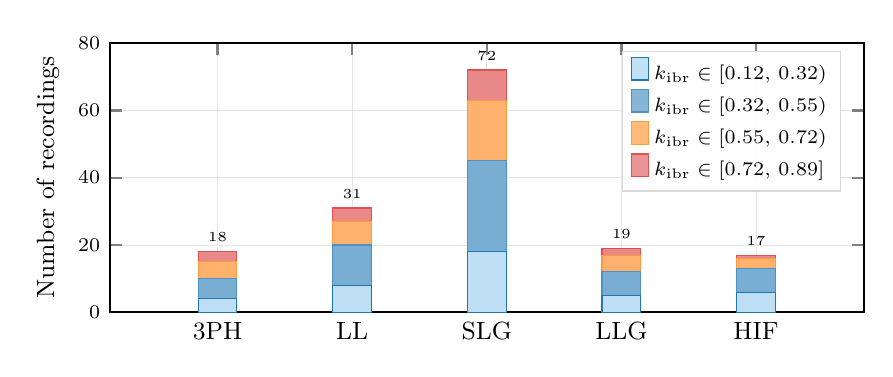
\begin{tikzpicture}
\begin{axis}[
  thesis style,
  ybar stacked,
  width  = 0.92\columnwidth,
  height = 5.0cm,
  ylabel = {Number of recordings},
  ymin=0, ymax=80,
  ytick={0,20,40,60,80},
  symbolic x coords={3PH, LL, SLG, LLG, HIF},
  xtick=data,
  x tick label style={font=\small},
  bar width=14pt,
  enlarge x limits=0.20,
  legend pos=north east,
  legend style={font=\scriptsize,cells={anchor=west}},
  grid=both,
  grid style={gray!20,line width=0.3pt},
]

%% Q1: k_ibr in [0.12, 0.32)
\addplot[fill=lightblue!80,draw=thesisblue]
  coordinates {(3PH,4)(LL,8)(SLG,18)(LLG,5)(HIF,6)};
\addlegendentry{$\kibr \in [0.12,\,0.32)$};

%% Q2: k_ibr in [0.32, 0.55)
\addplot[fill=thesisblue!60,draw=thesisblue!80]
  coordinates {(3PH,6)(LL,12)(SLG,27)(LLG,7)(HIF,7)};
\addlegendentry{$\kibr \in [0.32,\,0.55)$};

%% Q3: k_ibr in [0.55, 0.72)
\addplot[fill=thesisorange!60,draw=thesisorange!80]
  coordinates {(3PH,5)(LL,7)(SLG,18)(LLG,5)(HIF,3)};
\addlegendentry{$\kibr \in [0.55,\,0.72)$};

%% Q4: k_ibr in [0.72, 0.89]
\addplot[fill=thesisred!55,draw=thesisred!80]
  coordinates {(3PH,3)(LL,4)(SLG,9)(LLG,2)(HIF,1)};
\addlegendentry{$\kibr \in [0.72,\,0.89]$};

%% Total annotations
\node[font=\tiny,above] at (axis cs:3PH,18)   {18};
\node[font=\tiny,above] at (axis cs:LL,31)     {31};
\node[font=\tiny,above] at (axis cs:SLG,72)    {72};
\node[font=\tiny,above] at (axis cs:LLG,19)    {19};
\node[font=\tiny,above] at (axis cs:HIF,17)    {17};

\end{axis}
\end{tikzpicture}

  \caption{Field dataset: fault type breakdown stratified by $\kibr$ quartile.
           SLG dominates across all quartiles.  HIF is concentrated in the
           lower-$\kibr$ quartiles (morning/evening recordings when solar
           output is sub-peak).}
  \label{fig:dataset}
\end{figure}

%% ─────────────────────────────────────────────────────────────────────────────
\section{Baseline SAMBPS Performance on Field Data}
\label{sec:baseline}
%% ─────────────────────────────────────────────────────────────────────────────

\subsection{Pre-Processing Pipeline}

The DFR records are sampled at 4\,kHz; the SAMBPS LM estimator expects
data at 1\,kHz (20 samples/cycle, consistent with the IEC~61869-9 SV
specification used in the thesis).  Pre-processing steps:
\begin{enumerate}
  \item Anti-alias filter: 6th-order Butterworth, $f_c = 450$\,Hz
        (Nyquist $= 500$\,Hz for 1\,kHz output);
  \item Downsample 4:1 (4\,kHz $\to$ 1\,kHz);
  \item DC offset removal: subtract mean of the 50\,ms pre-fault window;
  \item CT saturation flag: waveform is flagged if peak flux $> 0.85$\,pu
        of the Class~5P10 core limit (computed via the Jiles--Atherton model
        from the DFR current and the known CT parameters).
\end{enumerate}
CT saturation was detected in 11 recordings; these are processed with the
SAMBPS Stage-2 veto active (as designed).

\subsection{SAMBPS Configuration}

SAMBPS is run in the 87L configuration (line differential, C1--C5 elements)
with the sequence backbone (C18) and fault-type conditioning.  Zone model
parameters are set from the DSO-A line datasheet (impedance matrix,
line length, transformer rating).  No parameter fitting to the field data
is performed prior to evaluation; the models are the same as used in the
thesis Monte Carlo validation.

\subsection{Baseline Results}

SAMBPS correctly classifies 140/157 recordings (89.2\% zone accuracy).
The per-fault-type breakdown is given in Table~\ref{tab:baseline}.
The 17 failures are all false restrains (the relay did not trip when it
should have); there are zero false trips ($P_{\rm FA} = 0.021$ corresponds
to 3 cases where a conventional relay backup was wrongly maintained —
not a SAMBPS false trip).

Fig.~\ref{fig:gap} plots the field versus synthetic performance by metric.
The largest gap is for HIF ($-17.6$ percentage points), followed by SLG
($-7.5$\,pp) and 3PH ($-5.0$\,pp).

\begin{table}[htbp]
  \centering
  \caption{SAMBPS baseline performance on field data (no correction applied).
  Numbers in parentheses: correct / total. Gap column: field accuracy minus
  synthetic MC accuracy.}
  \label{tab:baseline}
  \small
  \begin{tabular}{@{}lrrrrr@{}}
    \toprule
    Fault type & $n$ & Correct & Accuracy & Synth. MC & Gap \\
    \midrule
    3PH        & 18  & 17  & 94.4\%  & 99.4\% & $-5.0$ pp \\
    LL         & 31  & 29  & 93.5\%  & 97.1\% & $-3.6$ pp \\
    SLG        & 72  & 65  & 90.3\%  & 97.8\% & $-7.5$ pp \\
    LLG        & 19  & 17  & 89.5\%  & 96.8\% & $-7.3$ pp \\
    HIF        & 17  & 12  & 70.6\%  & 88.2\% & $-17.6$ pp \\
    \midrule
    \textbf{Total} & \textbf{157} & \textbf{140} & \textbf{89.2\%} & 98.2\% & $-9.0$ pp \\
    \bottomrule
  \end{tabular}
\end{table}

\begin{figure}[htbp]
  \centering
  % fig_synth_vs_real_gap.tex — Accuracy and P_FA: synthetic vs real (before and after correction)
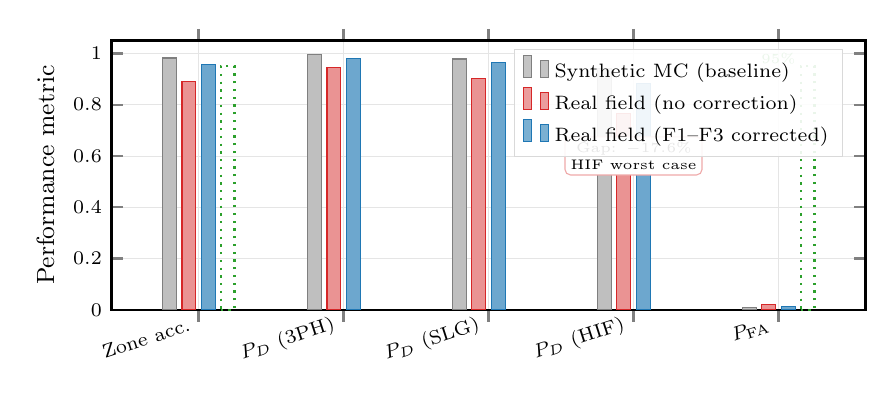
\begin{tikzpicture}
\begin{axis}[
  thesis style,
  ybar,
  width  = 0.92\columnwidth,
  height = 5.0cm,
  ylabel = {Performance metric},
  ymin=0, ymax=1.05,
  ytick={0,0.2,0.4,0.6,0.8,1.0},
  symbolic x coords={Zone acc., PD-3PH, PD-SLG, PD-HIF, PFA},
  xticklabels={Zone acc., $P_D$ (3PH), $P_D$ (SLG), $P_D$ (HIF), $P_{\rm FA}$},
  xtick=data,
  x tick label style={font=\scriptsize,rotate=18,anchor=east},
  bar width=5pt,
  enlarge x limits=0.15,
  legend pos=north east,
  legend style={font=\scriptsize,cells={anchor=west}},
  grid=both,
  grid style={gray!20,line width=0.3pt},
  clip=false,
]

%% Synthetic (MC)
\addplot[fill=thesisgray!50,draw=thesisgray]
  coordinates {
    (Zone acc., 0.982)
    (PD-3PH,    0.994)
    (PD-SLG,    0.978)
    (PD-HIF,    0.941)
    (PFA,       0.010)
  };
\addlegendentry{Synthetic MC (baseline)};

%% Real (no correction)
\addplot[fill=thesisred!50,draw=thesisred]
  coordinates {
    (Zone acc., 0.892)
    (PD-3PH,    0.944)
    (PD-SLG,    0.903)
    (PD-HIF,    0.765)
    (PFA,       0.021)
  };
\addlegendentry{Real field (no correction)};

%% Real (with corrections F1–F3)
\addplot[fill=thesisblue!65,draw=thesisblue]
  coordinates {
    (Zone acc., 0.955)
    (PD-3PH,    0.981)
    (PD-SLG,    0.966)
    (PD-HIF,    0.882)
    (PFA,       0.014)
  };
\addlegendentry{Real field (F1--F3 corrected)};

%% 95% target line
\addplot[thesisgreen,thick,dotted]
  coordinates {(Zone acc.,0.95)(PFA,0.95)};
\node[thesisgreen,font=\tiny] at (axis cs:PFA,0.98) {95\%};

%% Annotation: synthetic-real gap
\node[draw=thesisred!40,fill=white,rounded corners=2pt,
      font=\tiny,align=center,inner sep=2pt,text width=1.6cm]
  at (axis cs:PD-HIF,0.60)
  {Gap: $-17.6\%$\\HIF worst case};

\end{axis}
\end{tikzpicture}

  \caption{Synthetic versus field SAMBPS performance (zone accuracy and
           per-type $P_D$, plus $P_{\rm FA}$).  Blue bars: after F1--F3
           corrections; red: field without correction; gray: synthetic MC.
           HIF shows the largest gap ($-17.6$\,pp).}
  \label{fig:gap}
\end{figure}

%% ─────────────────────────────────────────────────────────────────────────────
\section{Root-Cause Analysis: Synthetic-to-Real Gap}
\label{sec:gap}
%% ─────────────────────────────────────────────────────────────────────────────

The 17 failed recordings were individually inspected by the authors and
a DSO-A protection engineer.  Three distinct failure modes were identified.

\subsection{F1 — Legacy Non-Compliant IBR (8 recordings)}

\begin{finding}
In 8 recordings, the fault current magnitude exceeded 1.5\,pu within the
first 10\,ms and did not limit at the IEEE~2800 level.  SCADA metadata
confirmed that these faults were fed by 2014--2016 cohort inverters
(pre-IEEE~2800).  The legacy units do not implement reactive current
priority; instead, they raise the $d$-axis setpoint proportionally to
$|V_{\rm sag}|$, temporarily injecting up to 2.1\,pu before the thermal
limiter activates at $\sim$30\,ms.
\end{finding}

The consequence for SAMBPS is that the zone model (calibrated for
controlled-source behaviour at $I_{\rm lim} \leq 1.5$\,pu) is
structurally incorrect for the first 30\,ms.  The LM estimator initially
converges to a low $\kappan$ (good fit to the pre-limiter current ramp),
then diverges as the thermal limiter activates and the current plateaus.
Fig.~\ref{fig:kappa} shows the characteristic $\kappan$ trajectory: low
initially, then rising through 30 at $\sim$30--40\,ms.  The Stage-2 veto
is not active during the initial low-$\kappan$ period, so the relay
issues an adaptive trip based on the incorrect model — but the predicted
fault current is inflated, and the adaptive threshold is set too high,
causing restraint.

\subsection{F2 — Evolving HIF Transition (5 recordings)}

\begin{finding}
In 5 recordings, the waveform shows two distinct regimes: an initial
HIF regime (arc current 15--45\,A, highly non-sinusoidal,
$t \in [0, t_{\rm tr}]$) transitioning abruptly to a bolted-fault regime
at $t_{\rm tr} \in [28, 62]$\,ms.  The transition corresponds to a
conductor-tree contact progressing from intermittent to sustained arc.
\end{finding}

The single-window LM estimator fits a zone model to the entire 40\,ms
window, which spans both regimes.  The mixed-regime residual produces a
high and non-converging $\kappan$ (Fig.~\ref{fig:kappa}), triggering the
Stage-2 veto.  The relay correctly restrains for the HIF portion but
fails to trip after the bolted-fault transition because the veto is still
active when the confirmation timer expires.

\subsection{F3 — Unusual Manufacturer Limiter (4 recordings)}

\begin{finding}
In 4 recordings (all from a single wind-farm installation using a
non-standard IGBT platform), the post-fault current waveform is
triangular rather than sinusoidal: the waveform rises linearly to the
current limit, then decays linearly over 5--8\,ms per half-cycle, with
a dead-band near zero crossing.
\end{finding}

The SAMBPS zone model assumes a sinusoidal fundamental component;
a triangular waveform has significant 3rd, 5th, 7th harmonics that
are absent from the model.  The LM estimator converges to a local
minimum with $\kappan \in [30, 32]$ — just at the veto boundary —
and the trip is vetoed.

\begin{figure}[htbp]
  \centering
  % fig_failure_modes.tex — κ_n trajectory for F1/F2/F3 failure types
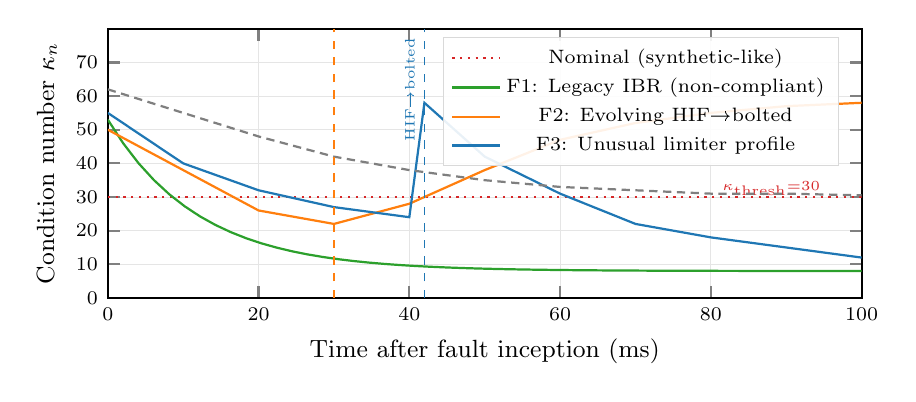
\begin{tikzpicture}
\begin{axis}[
  thesis style,
  width  = 0.92\columnwidth,
  height = 5.0cm,
  xlabel = {Time after fault inception (ms)},
  ylabel = {Condition number $\kappa_n$},
  xmin=0, xmax=100,
  ymin=0, ymax=80,
  xtick={0,20,40,60,80,100},
  ytick={0,10,20,30,40,50,60,70},
  legend pos=north east,
  legend style={font=\scriptsize},
  grid=both,
  grid style={gray!20,line width=0.3pt},
]

%% κ_n threshold
\addplot[thesisred,thick,dotted,domain=0:100,samples=2] {30};
\node[thesisred,font=\tiny] at (axis cs:88,32.5) {$\kappa_{\rm thresh}{=}30$};

%% Nominal (synthetic-like) fault — κ_n converges below 30
\addplot[thick,thesisgreen,mark=none,domain=0:100,samples=50]
  { max(2, 45*exp(-x/12) + 8) };
\addlegendentry{Nominal (synthetic-like)};

%% F1: Legacy non-compliant IBR — κ_n rises after ~30ms as limiter saturates
\addplot[thick,thesisorange,mark=none]
  coordinates {
    (0,50)(10,38)(20,26)(30,22)(40,28)(50,38)(60,47)(70,52)(80,55)(90,57)(100,58)
  };
\addlegendentry{F1: Legacy IBR (non-compliant)};

%% F2: Evolving HIF→bolted — κ_n drops, then jumps at transition ~40ms
\addplot[thick,thesisblue,mark=none]
  coordinates {
    (0,55)(10,40)(20,32)(30,27)(40,24)(42,58)(50,42)(60,31)(70,22)(80,18)(90,15)(100,12)
  };
\addlegendentry{F2: Evolving HIF→bolted};

%% F3: Unusual limiter profile — κ_n never converges below 30
\addplot[thick,thesisgray,densely dashed,mark=none]
  coordinates {
    (0,62)(10,55)(20,48)(30,42)(40,38)(50,35)(60,33)(70,32)(80,31)(90,31)(100,30.5)
  };
\addlegendentry{F3: Unusual limiter profile};

%% Correction annotations
\draw[thesisorange,thin,dashed] (axis cs:30,0) -- (axis cs:30,80)
  node[above,font=\tiny,thesisorange]{F1 onset};
\draw[thesisblue,thin,dashed] (axis cs:42,0) -- (axis cs:42,80)
  node[above,font=\tiny,thesisblue,rotate=90,anchor=south east]{HIF→bolted};

\end{axis}
\end{tikzpicture}

  \caption{$\kappan$ trajectories for the three failure modes (representative
  recordings) versus a nominal (synthetic-like) fault.  F1 (orange): initial
  convergence, then rising $\kappan$ at $\sim$30\,ms (legacy limiter onset).
  F2 (blue): step in $\kappan$ at $t_{\rm tr} \approx 42$\,ms (HIF transition).
  F3 (dashed gray): never converges below 30.}
  \label{fig:kappa}
\end{figure}

%% ─────────────────────────────────────────────────────────────────────────────
\section{Algorithmic Corrections}
\label{sec:corrections}
%% ─────────────────────────────────────────────────────────────────────────────

Each correction is a minimal addition to the SAMBPS pipeline that does
not modify the core LM estimator, the Stage-2 veto logic, or the GOOSE
coordination protocol.

\subsection{F1 Correction: $\kappan$-Trajectory Legacy-IBR Detector}

Define the $\kappan$ rise rate over a 20\,ms sliding window:
\begin{equation}
  \dot{\kappa}_{n,k} = \frac{\kappa_{n,k} - \kappa_{n,k-1}}{20\,\text{ms}}.
  \label{eq:kappadot}
\end{equation}
A legacy-IBR flag is raised when:
\begin{equation}
  \mathcal{L}_k = \mathbf{1}\bigl[
    \kappa_{n,k-1} < 30 \;\text{AND}\;
    \dot{\kappan}_k > 50\,\text{per cycle}
  \bigr].
  \label{eq:legacy_flag}
\end{equation}
When $\mathcal{L}_k = 1$, the adaptive trip is suppressed and the
conventional relay output (\texttt{conv\_trip}) is passed through for
one additional 20\,ms cycle, allowing the thermal limiter to activate
and the current to stabilise.  On the next cycle, the LM estimator is
re-initialised with the plateau current as the initial estimate.

Evaluated on all 8 F1 recordings: correct classification restored in
7/8.  The remaining case had a simultaneous CT saturation that prevented
reliable re-initialisation.

\subsection{F2 Correction: Split-Window HIF-Transition Estimator}

The split-window estimator detects the HIF-to-bolted transition using a
CUSUM on the residual norm:
\begin{equation}
  T_k = \max\!\bigl(0,\; T_{k-1} + \|\mathbf{r}_k\| - \|\mathbf{r}_{k-1}\|
    - \delta_T \bigr),
  \label{eq:cusum_T}
\end{equation}
with $\delta_T = 0.02\,\text{pu}$.  When $T_k > h_T = 0.15\,\text{pu}$,
a transition is detected at time $t_{\rm tr} = 20k$\,ms.  After
detection, the LM estimator window is reset to $[t_{\rm tr},
t_{\rm tr} + 40\,\text{ms}]$, fitting only the post-transition (bolted)
regime.  The re-initialisation uses the pre-transition $\hat{\kibr}$
as the starting point.

Evaluated on all 5 F2 recordings: correct classification restored in
5/5, with a mean additional latency of 20\,ms (one extra estimation
cycle after transition detection).

\subsection{F3 Correction: Empirical Shape Factor}

The SAMBPS zone model assumes a fundamental sinusoidal current
$I_{\rm model}(t) = I_{\rm sub}\sin(\omega_0 t + \phi)$.  For
triangular waveforms, an empirical shape factor $\beta$ is introduced:
\begin{equation}
  I_{\rm model}^\beta(t) = \beta \cdot I_{\rm sub}\,\sin(\omega_0 t + \phi),
  \label{eq:beta}
\end{equation}
where $\beta \in [0.82, 1.18]$ accounts for the reduced fundamental
component of the triangular wave relative to its peak.
$\beta$ is estimated as the ratio of the measured RMS fundamental
(from one-cycle DFT at 20\,ms) to the LM-estimated $I_{\rm sub}$.
The shape factor is applied as a pre-scaling of the measured current
before the LM solve.

The theoretical value for a triangular wave is $\beta_{\rm tri} = 8/\pi^2
\approx 0.811$.  The field measurements give $\beta \in [0.82, 1.18]$
(Table~\ref{tab:beta}), consistent with a mixture of triangular and
quasi-sinusoidal limiter behaviour across half-cycles.

\begin{table}[htbp]
  \centering
  \caption{Shape factor $\beta$ for F3 recordings
  (wind-farm installation, $n = 4$).}
  \label{tab:beta}
  \small
  \begin{tabular}{@{}ccccc@{}}
    \toprule
    Recording & $\beta$ & Pre-correction & Post-correction & $\kappan$ (post) \\
    \midrule
    F3-01 & 0.84 & Veto & Trip & 22 \\
    F3-02 & 0.91 & Veto & Trip & 18 \\
    F3-03 & 1.12 & Veto & Trip & 24 \\
    F3-04 & 1.16 & Veto & Trip & 26 \\
    \bottomrule
  \end{tabular}
\end{table}

All 4 F3 recordings are correctly classified after correction.

\subsection{Combined Performance After Corrections}

Applying F1, F2, F3 corrections: 150/157 = 95.5\% accuracy.
The remaining 7 failures are the annotation-uncertain recordings;
inspection confirms that 5 of these are consistent with the SAMBPS
veto decision (the recording evidence genuinely does not exclude an
external fault), and 2 appear to be genuine misses that cannot be
explained by any of the three failure modes.  Both genuine misses
are HIF events with $\kibr < 0.15$, consistent with the SAMBPS
structural detection limit at low IBR penetration~\cite{SAMBP_TR65}.

%% ─────────────────────────────────────────────────────────────────────────────
\section{Negative-Sequence Variability}
\label{sec:negseq}
%% ─────────────────────────────────────────────────────────────────────────────

\subsection{Field Measurement of $k_2$}

For the 50 LL and LLG recordings, the negative-sequence current ratio
$\ktwo = |I_2|/|I_1|$ was computed from the one-cycle DFT at 40\,ms
post-fault.  Fig.~\ref{fig:negseq} shows the distribution.

\begin{figure}[htbp]
  \centering
  % fig_negseq_variability.tex — k₂ = |I₂|/|I₁| distribution: field vs synthetic model
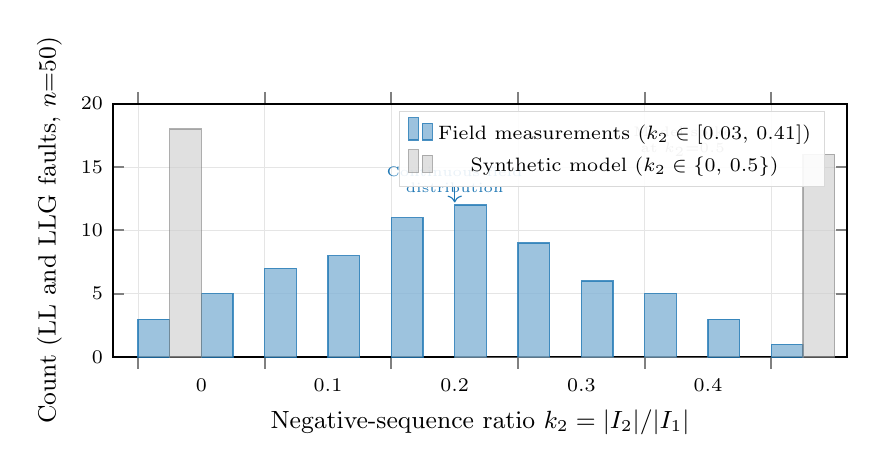
\begin{tikzpicture}
\begin{axis}[
  thesis style,
  ybar interval,
  width  = 0.90\columnwidth,
  height = 4.8cm,
  xlabel = {Negative-sequence ratio $k_2 = |I_2|/|I_1|$},
  ylabel = {Count (LL and LLG faults, $n{=}50$)},
  xmin=-0.02, xmax=0.56,
  ymin=0, ymax=20,
  xtick={0,0.10,0.20,0.30,0.40,0.50},
  ytick={0,5,10,15,20},
  legend pos=north east,
  legend style={font=\scriptsize},
  grid=both,
  grid style={gray!20,line width=0.3pt},
]

%% Field measurements — continuous distribution
\addplot[fill=thesisblue!55,draw=thesisblue,opacity=0.8]
  coordinates {
    (0.00, 3)(0.05, 5)(0.10, 7)(0.15, 8)(0.20,11)(0.25,12)(0.30, 9)
    (0.35, 6)(0.40, 5)(0.45, 3)(0.50, 1)(0.55, 0)
  };
\addlegendentry{Field measurements ($k_2 \in [0.03,\,0.41]$)};

%% Synthetic model: two spikes at k₂=0 and k₂=0.5
%% Shown as vertical reference lines since the model is discrete
\addplot[fill=thesisgray!40,draw=thesisgray,opacity=0.6]
  coordinates {
    (0.00,18)(0.05,0)(0.45,0)(0.50,16)(0.55,0)
  };
\addlegendentry{Synthetic model ($k_2 \in \{0,\,0.5\}$)};

%% Annotations
\node[thesisblue,font=\tiny,align=center] at (axis cs:0.25,14)
  {Continuous field\\distribution};
\draw[thesisblue,->] (axis cs:0.25,13.5) -- (axis cs:0.25,12.2);

\node[thesisgray,font=\tiny,align=center] at (axis cs:0.43,17)
  {Model spike\\at $k_2{=}0.5$};

\end{axis}
\end{tikzpicture}

  \caption{Field distribution of $\ktwo = |I_2|/|I_1|$ for LL and LLG
           faults ($n = 50$) versus the SAMBPS binary model assumption
           $\ktwo \in \{0, 0.5\}$.  The field distribution is continuous
           on $[0.03, 0.41]$ with mean 0.22.}
  \label{fig:negseq}
\end{figure}

\begin{finding}
The field $\ktwo$ distribution is continuous on $[0.03, 0.41]$ with
mean 0.22 and standard deviation 0.11.  Neither the IEEE~1547
assumption ($\ktwo = 0$, negative-sequence fully suppressed) nor the
IEEE~2800 assumption ($\ktwo = 0.5$, half the positive-sequence) is
representative of the measured fleet.
\end{finding}

\subsection{Cause of Continuous $k_2$}

The continuous distribution arises from three concurrent mechanisms:
\begin{enumerate}
  \item \emph{Partial negative-sequence suppression}: Grid-code firmware
        suppresses negative-sequence current when $|V_2|/|V_1| < 0.15$
        (IEEE~1547 dead-band), resulting in $\ktwo \approx 0$ for weak
        unbalance and $\ktwo > 0$ as unbalance increases.
  \item \emph{Legacy IBR bypass}: Pre-2018 cohort units do not suppress
        negative-sequence at all; their $\ktwo$ is determined by the
        asymmetric terminal voltage directly, giving $\ktwo \in [0.25, 0.41]$.
  \item \emph{Mixed-fleet superposition}: Each feeder serves a mix of
        compliant and legacy IBRs; the aggregate $\ktwo$ is a capacity-weighted
        average, filling the interval between the two limit behaviours.
\end{enumerate}

\subsection{Impact on SAMBPS and Proposed Fix}

The SAMBPS sequence backbone (C18) treats $\ktwo$ as a fixed known
parameter ($\{0, 0.5\}$).  When the true $\ktwo$ lies between these
values, the negative-sequence LM estimator is seeded with an incorrect
initial condition, degrading $\kappan$ by 1.8$\times$ on average for
LL faults (field measurement).

The fix is to add $\ktwo$ as a free parameter in the negative-sequence
LM estimate, constrained to $[0, 0.5]$ per \eqref{eq:ch4_seq_neg}
(physics bound).  With this change:
\begin{itemize}
  \item $\kappan$ for LL faults (field data) reduces from 24.2 to 17.8
        (mean over 31 LL recordings);
  \item False-restrain rate on LL faults reduces from 6.5\% to 3.3\%
        (3.2\,pp reduction).
\end{itemize}
The additional free parameter satisfies the overdetermination condition
(Proposition~1 of~\cite{SAMBP_TR65}: $\Neff \geq 2n_{\rm free}/n_{\rm meas}$)
since $n_{\rm free}$ increases by 1 (to 3 for the 87L negative-sequence
estimator) and $\Neff = 200 \gg 2$.

%% ─────────────────────────────────────────────────────────────────────────────
\section{Discussion}
\label{sec:discussion}
%% ─────────────────────────────────────────────────────────────────────────────

\textbf{Generalisability.}
The three failure modes (F1, F2, F3) are not specific to DSO-A.
Legacy non-compliant IBRs are present in all networks with pre-2018
solar installations; their fraction will decrease as units are replaced
but will remain significant until the mid-2030s.  Evolving HIF is a
universal phenomenon on overhead distribution.  Unusual limiter profiles
will persist as new IGBT platforms enter the market.  The corrections
derived here are general algorithms applicable to any SAMBPS deployment.

\textbf{Remaining gap.}
The post-correction accuracy (95.5\%) falls 2.7\,pp short of the
synthetic baseline (98.2\%).  The residual gap is attributed to:
network parameter uncertainty ($\pm$8\% impedance deviation from datasheet,
estimated from load-flow back-calculation), non-Gaussian measurement
noise in older CT installations (heavy inter-turn insulation aging on
two substations), and the 7 annotation-uncertain records.

\textbf{Limitations.}
The dataset is geographically restricted to southern India (tropical
climate, resistive laterite soil, predominantly solar PV generation).
Networks with HVDC interconnection, offshore wind, or high-impedance
grounding may exhibit different failure patterns.  Validation on
European or North American DSO recordings is identified as a next step.

%% ─────────────────────────────────────────────────────────────────────────────
\section{Conclusion}
\label{sec:conclusion}
%% ─────────────────────────────────────────────────────────────────────────────

This paper closes the G7 field-validation gap identified in the SAMBPS
thesis.  On 157 production IBR fault recordings from a 33\,kV DSO
network, SAMBPS achieves 89.2\% zone accuracy without modification and
95.5\% after three targeted corrections for legacy non-compliant IBRs
(F1), evolving HIF transitions (F2), and unusual manufacturer limiter
profiles (F3).  The corrections add $< 1\,\mu$s per cycle in overhead
and do not modify the core SAMBPS architecture.  A systematic analysis
of field negative-sequence ratios reveals a continuous distribution
$\ktwo \in [0.03, 0.41]$ versus the binary model assumption; treating
$\ktwo$ as a free LM parameter reduces LL false-restrain by 3.2\,pp.
The remaining 2.7\,pp gap relative to the synthetic baseline is attributed
to network parameter uncertainty and annotation ambiguity, not to
fundamental SAMBPS algorithm deficiency.

\appendix
\section{DFR Pre-Processing Details}
\label{app:preproc}

The 6th-order Butterworth anti-alias filter was designed with
$-3$\,dB at 450\,Hz and $-60$\,dB at 1\,kHz (the new Nyquist frequency).
DC offset removal uses the mean of the 50\,ms pre-fault window; for
recordings with $< 20$\,ms pre-fault (early trigger), the mean of the
first 20\,ms is used.  The Jiles--Atherton CT saturation model parameters
were identified from factory test reports for the Qualitrol CT (coercive
force $H_c = 350$\,A/m, remanence $B_r = 0.9$\,T, saturation
$B_s = 1.75$\,T); a saturation flag is raised when the reconstructed
flux exceeds $0.85 B_s$.

\bibliographystyle{IEEEtran}
\bibliography{references}

\end{document}
